% Nome do capítulo
\chapter{Metodologia}
% Label para referenciar
\label{ch:meto}

% Diminuir espaçamento entre título e texto
\vspace{-1.9cm}
Os componentes utilizados para a execução desse projeto são um \textit{Arduino Mega 2560}, 14 sensores de flexão, e duas \ac{IMU}s \textit{MPU-9250}. O motivo da escolha destes componentes será explicado na Seção \ref{sec:hardware}.

Para a execução desse projeto foi construído um novo protótipo baseado na luva de \citeonline{roversi} (Figura \ref{fig:luvaorig}), que possui as seguintes limitações:

\begin{compactitem}
  \item[a)] não detecta movimentos de adução e abdução dos dedos;
  \item[b)] não detecta movimentos de desvio radial e ulnar do pulso;
  \item[c)] ruídos provenientes da \ac{IMU} utilizada;
  \item[d)] sensores de flexão não estão propriamente posicionados.
\end{compactitem}

Para solucionar o problema da detecção dos movimentos de adução e abdução, foram utilizados mais quatro sensores de flexão posicionados entre cada par dedos. Os dados gerados por esses sensores foram transformados no ângulo de abertura formado entre os dedos e fornecidos ao \textit{script} da \textit{Unity} para animação do modelo \ac{3D} da mão. Para captura dos dados de orientação da mão foram utilizadas duas \ac{IMU}s \textit{MPU-9250}, uma nas costas da mão e outra acima do pulso, no antebraço, de modo que as diferenças entre os ângulos de orientação das duas \ac{IMU}s fornecessem o ângulo de dobra entre o pulso e o antebraço, o que corresponderia aos movimentos de desvio radial e ulnar do pulso. A Figura \ref{fig:novaluva} mostra o diagrama de posicionamento dos componentes na luva para a solução dos problemas propostos.

O sinal de orientação que é enviado pelo \textit{Arduino} é bastante ruidoso, causando instabilidade no modelo \ac{3D} e fazendo-o tremer. Tal ruído é proveniente do acelerômetro, pois este é impreciso para fornecer dados do ângulo de orientação do sensor, portanto leituras somente do acelerômetro não podem ser utilizadas. Por outro lado, o giroscópio fornece dados estáveis de ângulo, mas pequenos erros de leitura acumulam-se com o tempo, fornecendo dados incorretos (efeito conhecido como \textit{drift}). A solução é utilizar as leituras do acelerômetro e do giroscópio em conjunto para obter valores mais próximos dos reais. A \ac{IMU} \textit{MPU-9250} possui um processador interno chamado de \ac{DMP} que realiza a fusão e filtragem dos dados do acelerômetro, giroscópio e magnetômetro e fornece a orientação da \ac{IMU} sem a necessidade de utilizar o processador do \textit{Arduino} para isso.

\begin{figure}[H]
  \setlength{\abovecaptionskip}{0pt}
  \setlength{\belowcaptionskip}{0pt}
  \caption[Diagrama da Luva]{Diagrama da Luva}
  \centering
  \subfloat[Protótipo original]{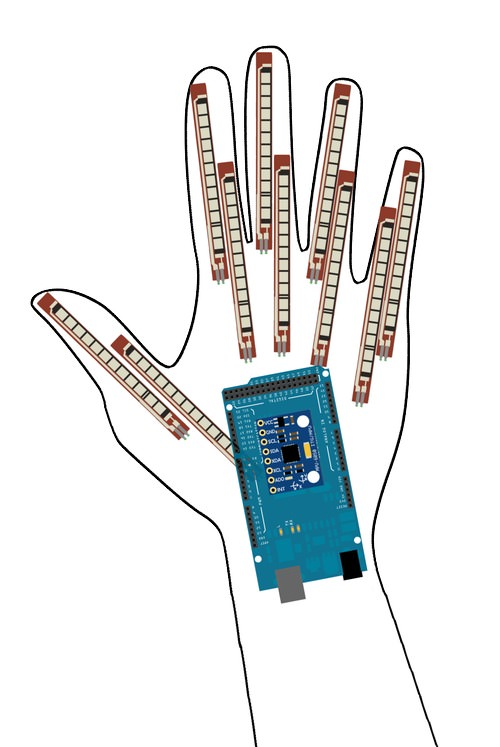
\includegraphics[width=.45\textwidth]{imagem/Luva_Atual}\label{fig:luvaorig}}
  \subfloat[Novo protótipo]{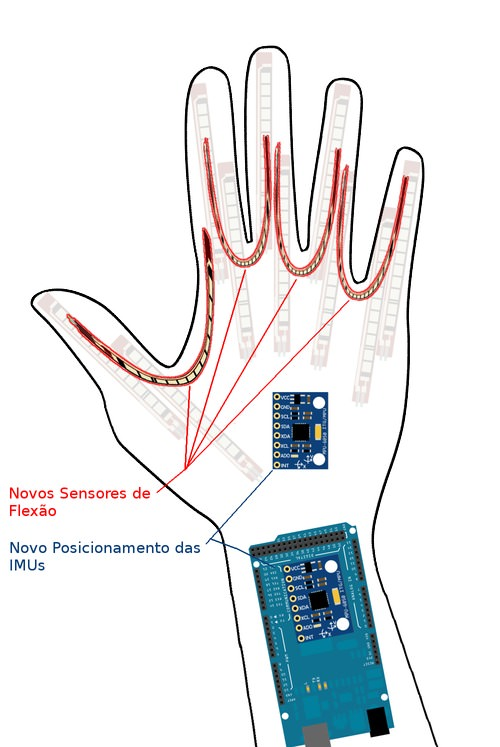
\includegraphics[width=.45\textwidth]{imagem/Nova_Luva}\label{fig:novaluva}}
  \captionsetup{justification=centering}
  \captionfont{\small{\textbf{\\Fonte: Elaborado pelo Autor}}}
  \label{fig:diagluva}
\end{figure}

A verificação do funcionamento correto da luva e análise da redução de ruídos foi feita observando os valores da média, \ac{DP}, amplitude e \ac{DMA} dos valores brutos recebidos dos sensores.

\section{Diagrama de Arquitetura}
\label{sec:arquitetura}
O diagrama da Figura \ref{fig:arq} representa a arquitetura do projeto, mostrando as conexões entre cada componente. O \textit{Arduino} lê os dados de dobra dos sensores de flexão e os dados de orientação das duas \ac{IMU}s e os envia através de um cabo \ac{USB} para o computador.

\begin{figure}[H]
  \setlength{\abovecaptionskip}{0pt}
  \setlength{\belowcaptionskip}{0pt}
  \caption[Diagrama de arquitetura]{Diagrama de arquitetura}
  \centering
  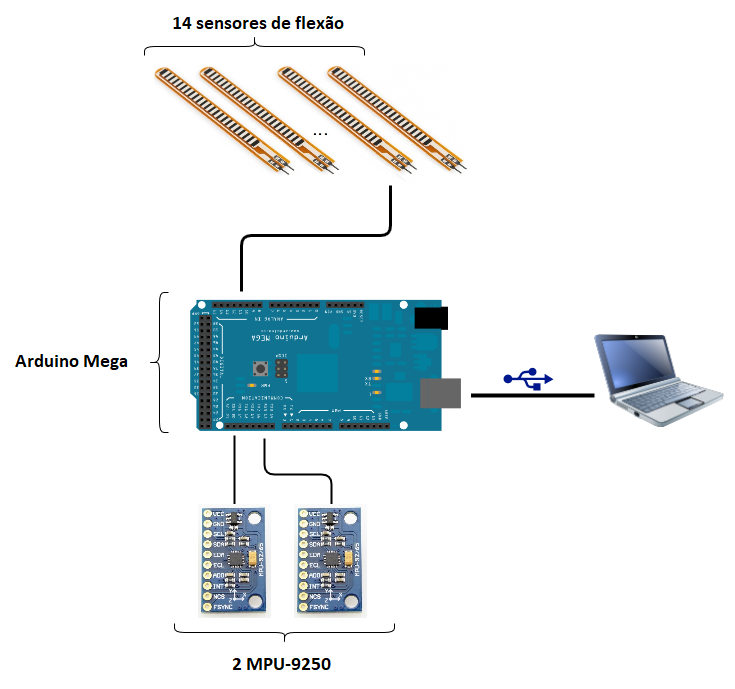
\includegraphics[width=.7\textwidth]{imagem/arquitetura}
  \captionsetup{justification=centering}
  \captionfont{\small{\textbf{\\Fonte: Elaborado pelo Autor}}}
  \label{fig:arq}
\end{figure}

\section{Diagrama de Caso de Uso}
\label{sec:caso_de_uso}
A Figura \ref{fig:uml} apresenta o diagrama de caso de uso do projeto, representando o fluxo de troca de dados entre usuário, \textit{Arduino} e \textit{Unity}.

Primeiro o usuário movimenta a luva, gerando as leituras de ângulos de dobra dos dedos e ângulo de orientação da mão e do braço. Em seguida o \textit{Arduino} recebe esses dados e os prepara para envio pela porta serial do computador para a aplicação \textit{Unity}, que requisita esses dados a cada atualização de \textit{frame}.

\begin{figure}[H]
  \setlength{\abovecaptionskip}{0pt}
  \setlength{\belowcaptionskip}{0pt}
  \caption[Diagrama de caso de uso]{Diagrama de caso de uso}
  \centering
  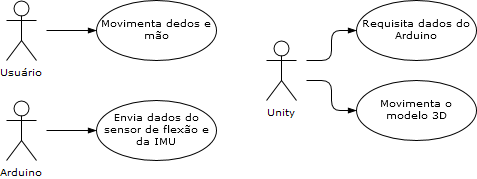
\includegraphics[width=.7\textwidth]{imagem/Caso_de_Uso}
  \captionsetup{justification=centering}
  \captionfont{\small{\textbf{\\Fonte: Elaborado pelo Autor}}}
  \label{fig:uml}
\end{figure}

\section{Diagrama de Sequência}
\label{sec:sequencia}
O diagrama de sequência mostrado na Figura \ref{fig:seq} exibe a sequência de troca de dados entre sensores \textit{Arduino} e \textit{Unity}, desde a captação dos dados até a exibição do resultado na tela. Também é possível observar que os dados mais recentes só são enviados à \textit{Unity} quando ocorre a atualização do \textit{frame}. Isso foi feito para evitar que os valores dos sensores fiquem presos no \textit{buffer} de entrada da porta serial, o que pode resultar em uma resposta lenta do modelo \ac{3D}.

A movimentação da mão do usuário gera as leituras de dobra dos dedos e posição da mão em relação ao braço. Os valores de dobra são lidos pelo \textit{Arduino} através da função \lstinline!Analog.read()! e os valores dos ângulos de orientação da mão são recebidos pelo \textit{Arduino} através da função \lstinline!mpu.dmpGetQuaternion()! do \textit{MPU-9250}. Durante cada atualização de \textit{frame} da \textit{Unity}, é enviado um caractere pela porta serial que serve para requisição dos dados atuais dos sensores. O \textit{Arduino} então lê esse caractere e envia os dados pela porta serial para a \textit{Unity}, que os usa para manipular os objetos na tela através da função \lstinline!transform.localEulerAngles()!.

\begin{figure}[H]
  \setlength{\abovecaptionskip}{0pt}
  \setlength{\belowcaptionskip}{0pt}
  \caption[Diagrama de sequência]{Diagrama de sequência}
  \centering
  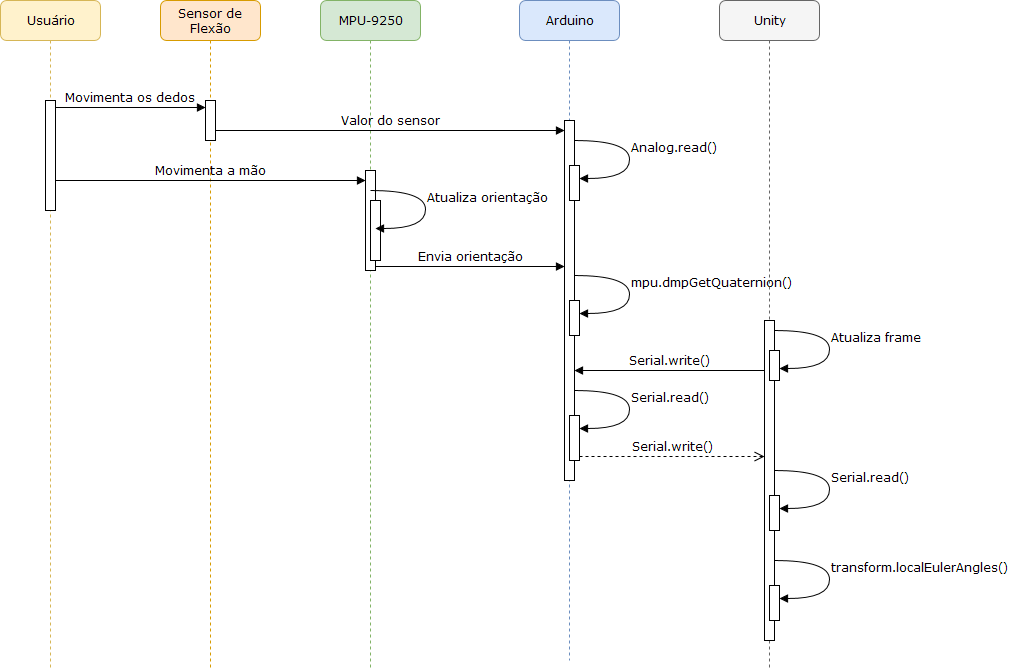
\includegraphics[width=\textwidth]{imagem/sequencia}
  \captionsetup{justification=centering}
  \captionfont{\small{\textbf{\\Fonte: Elaborado pelo Autor}}}
  \label{fig:seq}
\end{figure}

\section{Requisitos}
\label{sec:requisitos}
Os requisitos foram definidos com o intuito de definir o escopo do trabalho, prover uma base para realização de testes e ajudar a verificar o funcionamento correto do dispositivo, quando concluído.

Os requisitos de \textit{hardware} para este projeto são:

\begin{compactitem}
  \item[a)] detectar os movimentos de adução e abdução dos dedos de $\pm$ \ang{15};
  \item[b)] detectar os movimentos de desvio radial e ulnar do pulso de $\pm$ \ang{20};
  \item[c)] nenhum componente da luva poderá impedir algum movimento da mão usuário.
\end{compactitem}

A escolha dos valores dos ângulos de abdução e desvio radial e ulnar do pulso foram baseadas nos limites dos movimentos da mão humana (\cite{hand_motions}).

Os requisitos de \textit{software} para este projeto são:

\begin{compactitem}
  \item[a)] reprodução dos movimentos dos dedos do usuário pelo modelo \ac{3D};
  \item[b)] rotação do modelo \ac{3D} de acordo com a orientação da mão do usuário;
  \item[c)] movimentos suaves do modelo \ac{3D}.
\end{compactitem}

\section{\textit{Hardware}}
\label{sec:hardware}

Nesta seção serão apresentados os componentes de \textit{hardware} que serão utilizados para a execução do projeto.

\subsection{Arduino}
\label{sub:arduino}
Assim como no trabalho de \citeonline{roversi}, foi mantida a plataforma \textit{Arduino} para desenvolvimento do projeto. Os principais motivos dessa escolha foram a grande quantidade disponível de módulos, \textit{shields} e sensores, e sua ativa comunidade de desenvolvimento, disponibilizando documentação e bibliotecas para estes dispositivos. Um outro fator que contribuiu para essa decisão foi a facilidade de desenvolver protótipos nessa plataforma.

Para esse projeto, optou-se por utilizar o \textit{Arduino Mega 2560}, devido ao fato de possuir a quantidade necessária de entradas analógicas para conexão com os sensores de flexão, já que serão utilizados 14 sensores e este modelo possui 16 entradas analógicas, como especificado na Tabela \ref{tab:ardspec}. A Figura \ref{fig:arduino} apresenta o \textit{Arduino Mega 2560} que foi utilizado para leitura dos dados dos sensores e comunicação com o computador.

\begin{figure}[H]
  \setlength{\abovecaptionskip}{0pt}
  \setlength{\belowcaptionskip}{0pt}
  \caption[\textit{Arduino Mega 2560}]{\textit{Arduino Mega 2560}}
  \centering
  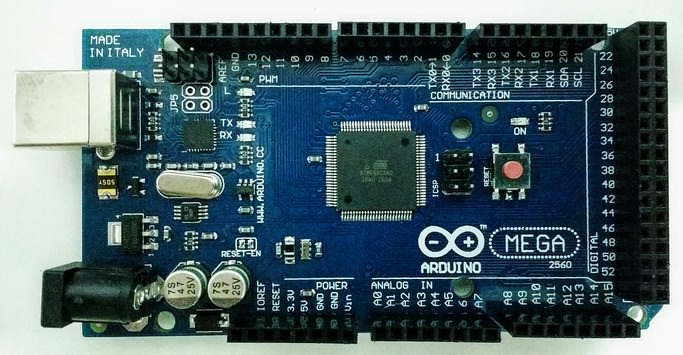
\includegraphics[width=0.5\textwidth]{imagem/ArduinoMega2560R3}
  \captionsetup{justification=centering}
  \captionfont{\small{\textbf{\\Fonte: Elaborado pelo Autor}}}
  \label{fig:arduino}
\end{figure}

\begin{table}[H]
  \centering
  \footnotesize
  \setlength{\abovecaptionskip}{0pt}
  \setlength{\belowcaptionskip}{0pt}
  \caption[Especificações do \textit{Arduino Mega 2560}]{Especificações do \textit{Arduino Mega 2560}}
  \label{tab:ardspec}
  \begin{tabular}{l l}
    \hline\hline
    Microcontrolador                & ATmega2560 \\
    Tensão de Operação              & \SI{5}{\volt} \\
    Tensão de entrada (recomendada) & \SIrange[range-phrase = --]{7}{12}{\volt} \\
    Tensão de entrada (limite)      & \SIrange[range-phrase = --]{6}{20}{\volt} \\
    Pinos de E/S Digital            & 54 (15 com saída PWM) \\
    Pinos de Entrada Analógica      & 16 \\
    Corrente DC por Pino de E/S     & \SI{20}{\milli\ampere} \\
    Corrente DC por Pino 3.3V       & \SI{50}{\milli\ampere} \\
    Memória \textit{Flash}          & \SI{256}{\kilo\byte} (\SI{8}{\kilo\byte} utilizados pelo \textit{bootloader}) \\
    SRAM                            & \SI{8}{\kilo\byte} \\
    EEPROM                          & \SI{4}{\kilo\byte} \\
    \textit{Clock}                  & \SI{16}{\mega\hertz} \\
    Comprimento                     & \SI{101.52}{\mm} \\
    Largura                         & \SI{53.3}{\mm} \\
    Peso                            & \SI{37}{\gram} \\
    \hline\hline
  \end{tabular}
  \\\vspace{1.3mm}
  \captionfont{\small{\textbf{Fonte: \citeonline{arduino}}}}
\end{table}

\subsection{Sensor Flexão}
\label{sub:sensorflexão}
Para a leitura dos movimentos dos dedos, optou-se por continuar a utilizar o sensor de flexão de 2.2" da \textit{Spectra Symbol}, devido ao fato de ser leve, não intrusivo para o usuário, simples de utilizar e fornecer resultados satisfatórios. A Figura \ref{fig:spectraflex} apresenta o sensor de flexão utilizado e a Tabela \ref{tab:flexspec} mostra suas especificações técnicas.

Foram utilizados 14 sensores, sendo dois sensores por dedo para captar os movimentos de flexão e extensão e 4 sensores entre cada dedo, detectando movimentos de adução e abdução. A disposição dos sensores na luva está representada na Figura \ref{fig:novaluva}. Foi utilizado apenas um sensor para detectar as dobras da segunda e terceira falanges para simplificar a construção da luva e reduzir custos. O ângulo de dobra da terceira falange pode ser calculado a partir do ângulo de de dobra da segunda falange (\cite{li2009smartglove}).

\begin{table}[H]
  \centering
  \footnotesize
  \setlength{\abovecaptionskip}{0pt}
  \setlength{\belowcaptionskip}{0pt}
  \caption[Especificações do Sensor de Flexão]{Especificações do Sensor de Flexão}
  \label{tab:flexspec}
  \begin{tabular}{l l}
    \hline\hline
    Ciclo de vida             & > 1 milhão \\
    Altura                    & \SI{0.43}{\mm} \\
    Comprimento ativo         & \SI{55.37}{\mm} \\
    Largura                   & \SI{6.35}{\mm} \\
    Variação de temperatura   & \SIrange{-35}{+80}{\degreeCelsius} \\
    Resistência plano         & \SI{25}{\kilo\ohm} \\
    Tolerância da resistência & \SI{+-30}{\percent} \\
    Variação de Resistência   & \SIrange{45}{125}{\kilo\ohm} (depende do raio de dobra) \\
    Potência                  & \SI{0.50}{\watt} contínuos. Pico \SI{1}{\watt} \\
    \hline\hline
  \end{tabular}
  \\\vspace{1.3mm}
  \captionfont{\small{\textbf{Fonte: \citeonline{symbol2012flex}}}}
\end{table}

\begin{figure}[H]
  \setlength{\abovecaptionskip}{0pt}
  \setlength{\belowcaptionskip}{0pt}
  \caption[Sensor de Flexão Spectra Symbol]{Sensor de Flexão Spectra Symbol}
  \centering
  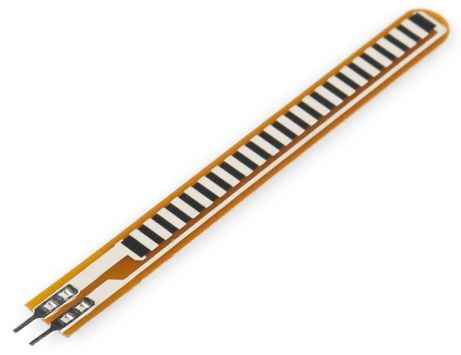
\includegraphics[width=0.4\textwidth]{imagem/spectraFlex}
  \captionsetup{justification=centering}
  \captionfont{\small{\textbf{\\Fonte: \citeonline{sparkflex}}}}
  \label{fig:spectraflex}
\end{figure}

\subsection{\ac{IMU}}
\label{sub:mpu}
Para a leitura da orientação da mão, foi utilizado a \ac{IMU} \textit{MPU-9250} da \textit{InvenSense} (Figura \ref{fig:mpu9250}). A escolha dessa \ac{IMU} deu-se primariamente pelo fato de ser acessível e possuir 9 \ac{DOF}, ou seja, consegue detectar movimentos de translação e rotação sobre qualquer um dos três eixos do espaço com maior precisão, fazendo uso de um acelerômetro, um giroscópio e um magnetômetro. Como especificado na Tabela \ref{tab:mpuspec}, o circuito do \textit{MPU-9250} possui comunicação através do protocolo \ac{I2C}, tornando sua utilização simples e permitindo a conexão de dois ou mais \ac{IMU} com apenas duas conexões (\ac{SDA} e \ac{SCL}) no \textit{Arduino}.

Foi utilizada a biblioteca \textit{I\textsuperscript{2}Cdevlib} \cite{i2c}, que possui funções para comunicação com diversos dispositivos que utilizam a interface I\textsuperscript{2}C (\ac{I2C}), como a \ac{IMU} em questão. Essa biblioteca possibilita a ativação e utilização do \ac{DMP} do \textit{MPU-9250}, que faz operações matemáticas complexas para combinar as leituras do acelerômetro, giroscópio e magnetômetro sem a utilização do processador do \textit{Arduino}, e fornecer dados confiáveis e livres de ruído que serão utilizados para calcular a orientação da \ac{IMU} no espaço.

\begin{figure}[H]
  \setlength{\abovecaptionskip}{0pt}
  \setlength{\belowcaptionskip}{0pt}
  \caption[\ac{IMU} MPU-9250]{\ac{IMU} MPU-9250}
  \centering
  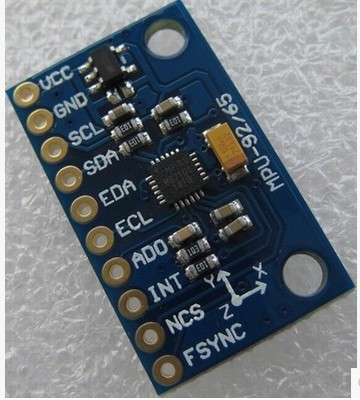
\includegraphics[height=5cm]{imagem/mpu9250}
  \captionsetup{justification=centering}
  \captionfont{\small{\textbf{\\Fonte: \citeonline{mpu9250}}}}
  \label{fig:mpu9250}
\end{figure}

\begin{table}[H]
  \centering
  \footnotesize
  \setlength{\abovecaptionskip}{0pt}
  \setlength{\belowcaptionskip}{0pt}
  \caption[Especificações do IMU \textit{MPU-9250}]{Especificações do IMU \textit{MPU-9250}}
  \label{tab:mpuspec}
  \begin{tabular}{l l}
    \hline\hline
    Tensão de operação (VDD)    & \SIrange[range-phrase = --]{2.4}{3.6}{\volt} \\
    Tensão lógica (VDDIO)       & \SI{1.7}{\volt} a VDD, ou VDD \\
    Saída Digital               & I\textsuperscript{2}C / SPI \\
    Sensibilidade Acelerômetro  & \SI[per-mode=fraction]{+-4800}{LSB\per\g} \\
    Gama Acelerômetro           & \SI{+-2}, \SI{+-4}, \SI{+-8}, \SI{+-16}{LSB\per\g} \\
    Taxa de Ruído do Giroscópio & \SI{+-4800}{\micro\farad} \\
    Gama Giroscópio             & \SI{+-250}, \SI{+-500}, \SI{+-1000}, \SI[per-mode=symbol]{+-2000}{\degree\per\second} \\
    Dimensões do Componente   & \SI[product-units = single]{3 x 3 x 1}{\mm}\\
    \hline\hline
  \end{tabular}
  \\\vspace{1.3mm}
  \captionfont{\small{\textbf{Fonte: \citeonline{specmpu9250}}}}
\end{table}

\subsection{Circuito}
\label{sub:circuito}
O Apêndice \ref{apend:circ} apresenta o diagrama elétrico completo do circuito do projeto. Como mostrado na Tabela \ref{tab:listacomponentes} foram utilizados 14 sensores de flexão que estão conectados às entradas analógicas do \textit{Arduino} como mostra a Figura \ref{fig:circsens}, com 14 resistores de \SI{10}{\kilo\ohm} fazendo um divisor de tensão para obter os dados dos sensores. De acordo com a Figura \ref{fig:circimu}, as duas \ac{IMU}s foram conectadas nos pinos \ac{SCL} e \ac{SDA} da interface \ac{I2C} e, seus pinos \ac{INT} conectados aos pinos digitais 2 e 3 do \textit{Arduino} que são os pinos 6 e 7 do \textit{ATmega 2560}, representados na Figura \ref{fig:circard}. Os pinos AD0 das \ac{IMU}s foram conectados em \SI{3.3}{\volt} e \ac{GND} para que possam ter endereços diferentes no barramento \ac{I2C}. A comunicação entre o computador e o \textit{Arduino} foi feita através de um cabo \ac{USB}.

\begin{table}[H]
  \centering
  \footnotesize
  \setlength{\abovecaptionskip}{0pt}
  \setlength{\belowcaptionskip}{0pt}
  \caption[Lista de Componentes]{Lista de Componentes}
  \label{tab:listacomponentes}
  \begin{tabular}{l r}
    \hline\hline
    \multicolumn{1}{c}{Componente}&\multicolumn{1}{c}{Quantidade}\\
    \hline
    \textit{Arduino Mega}           & 1 \\
    \textit{MPU-9250}               & 2 \\
    Conectores em barra de 40 pinos & 1 \\
    \textit{Shield} de Prototipagem para \textit{Arduino} & 1 \\
    Sensores de flexão              & 14 \\
    Resistores (\SI{10}{\kilo\ohm}) & 14 \\
    Fios & 40\\
    \hline\hline
  \end{tabular}
  \\\vspace{1.3mm}
  \captionfont{\small{\textbf{Fonte: Elaborado pelo Autor}}}
\end{table}

\begin{figure}[H]
  \setlength{\abovecaptionskip}{0pt}
  \setlength{\belowcaptionskip}{0pt}
  \caption[Detalhes do circuito elétrico]{Detalhes do circuito elétrico}
  \centering
  \subfloat[Conexões Sensores]{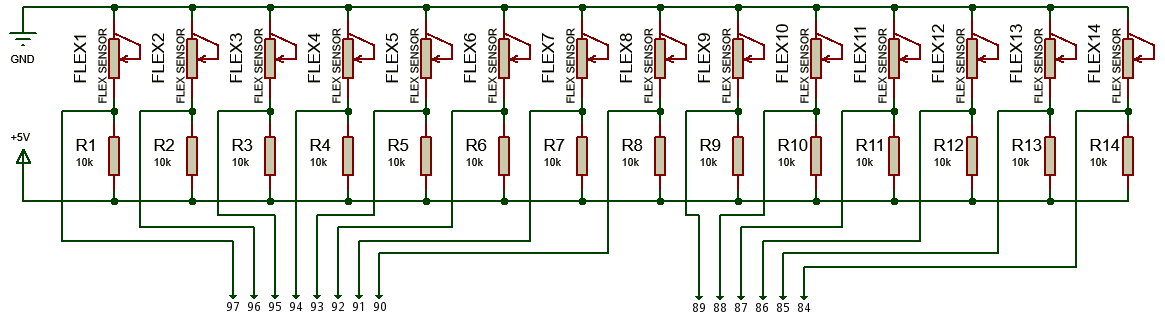
\includegraphics[width=\textwidth]{imagem/ProteusLuvaSensores}\label{fig:circsens}}\\
  \subfloat[Conexões \textit{Arduino}]{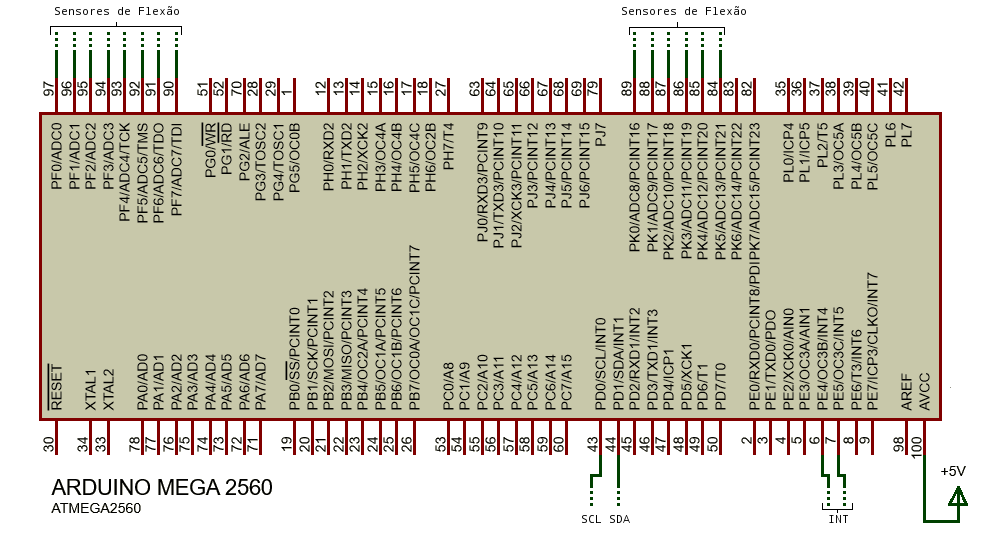
\includegraphics[width=\textwidth]{imagem/ProteusLuvaArduino}\label{fig:circard}}\\
  \label{fig:circLuva1}
  \captionsetup{justification=centering}
  \captionfont{\small{\textbf{\\Fonte: Elaborado pelo Autor}}}
\end{figure}

\begin{figure}[H]
\ContinuedFloat
  \setlength{\abovecaptionskip}{0pt}
  \setlength{\belowcaptionskip}{0pt}
  \caption[Detalhes do circuito elétrico]{Detalhes do circuito elétrico}
  \centering
  \subfloat[Conexões \ac{IMU}s]{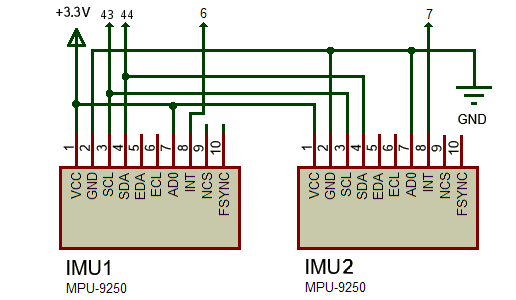
\includegraphics[width=.5\textwidth]{imagem/ProteusLuvaIMU}\label{fig:circimu}}\\
  \label{fig:circLuva2}
  \captionsetup{justification=centering}
  \captionfont{\small{\textbf{\\Fonte: Elaborado pelo Autor}}}
\end{figure}

\section{\textit{Software}}
\label{sec:software}

Nesta seção serão apresentados os \textit{softwares} que foram utilizados para a execução do projeto.

\subsection{Unity}
\label{sub:unity}
Para animação e exibição do modelo \ac{3D}, optou-se pela utilização da plataforma \textit{Unity}, versão 5.6.2, que é um ambiente para desenvolvimento para jogos digitais. A escolha dessa plataforma deu-se com base em sua facilidade de aprendizado e utilização, e também na grande variedade de modelos \ac{3D} disponibilizados por sua comunidade.

O modelo de mão e braço \ac{3D} utilizado foi o mesmo de \citeonline{roversi} (Figura \ref{fig:maounity}). Para a movimentação do modelo, foi implementado um \textit{script} em \csharp que recebe os dados de cada sensor provenientes do \textit{Arduino} e aplica as transformações dos dedos e na rotação da mão \ac{3D}.

A aplicação \textit{Unity} exibe a representação da mão do usuário em um modelo \ac{3D} que replica os movimentos realizados.

\begin{figure}[H]
  \setlength{\abovecaptionskip}{0pt}
  \setlength{\belowcaptionskip}{0pt}
  \caption[Tela da aplicação Unity]{Tela da aplicação Unity}
  \centering
  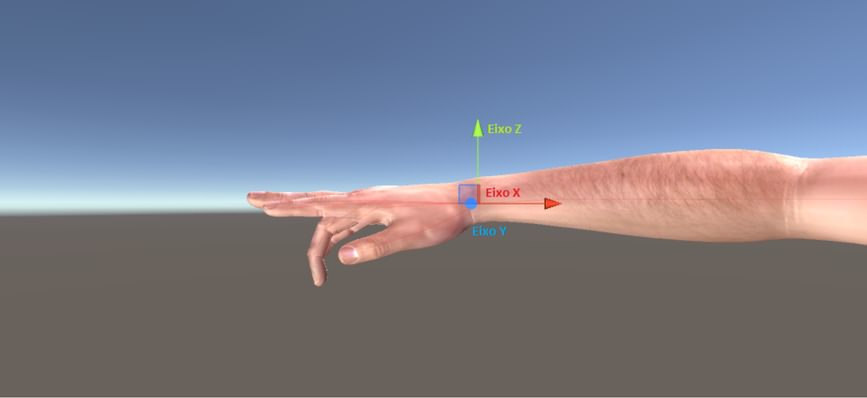
\includegraphics[trim=40 20 40 20,clip,width=.5\textwidth]{imagem/maoUnity}
  \captionsetup{justification=centering}
  \captionfont{\small{\textbf{\\Fonte: \citeonline{roversi}}}}
  \label{fig:maounity}
\end{figure}

\section{Plataforma de Desenvolvimento}
\label{sub:plataforma_de_desenvolvimento}
Este trabalho foi desenvolvido em um \textit{notebook} \textit{HP}, modelo \textit{G71}. Suas especificações são mostradas na Tabela \ref{tab:especificacoes} abaixo:

\begin{table}[H]
  \centering
  \footnotesize
  \setlength{\abovecaptionskip}{0pt}
  \setlength{\belowcaptionskip}{0pt}
  \caption[Especificações da plataforma de desenvolvimento]{Especificações da plataforma de desenvolvimento}
  \label{tab:especificacoes}
    \begin{tabular}{l l}
    \hline\hline
    Processador         & \textit{Intel Core 2 Duo T6600} \SI{2.20}{\giga\hertz} \\
    Memória             & \SI{4}{\giga\byte}\\
    Placa de vídeo      & \textit{Intel Graphics Media Accelerator 4500MHD} \\
    Disco Rígido        & \SI{320}{\giga\byte} (5400RPM) \\
    Sistema Operacional & \textit{Windows 10} \SI{64}{\bit} \\
    \hline\hline
  \end{tabular}
  \\\vspace{1.3mm}
  \captionfont{\small{\textbf{Fonte: Elaborado pelo Autor}}}
\end{table}

\subsection{Casos de Teste}
\label{sub:testes}

Para a comparação dos dois protótipos, foi utilizada uma abordagem semelhante à de \citeonline{li2009smartglove}, onde foram realizadas uma série de medições do ângulo de dobra real dos dedos e comparada com o valor lido pelo sensor após as devidas conversões. A precisão dos resultados foi avaliada utilizando \ac{DMA} dado pela Equação \ref{eq:dma}: 

\begin{equation} \label{eq:dma}
	DMA = \frac{1}{n}\sum_{i=1}^n\lvert V_r - V_c \rvert
\end{equation}

Onde $n$ é o número de amostras, $V_r$ é o valor real do ângulo de dobra e $V_c$ é o valor do ângulo calculado pelo \textit{Arduino}. Idealmente os valores medidos e calculados deveriam ser iguais, ou seja, $V_r=V_c$, fazendo com que $DMA=0$, mas devido às imprecisões tanto nos sensores, quanto no processo de conversão, isso não ocorre. Portanto é desejável que o valor do \ac{DMA} seja o mais próximo de $0$.

O novo protótipo também foi analisado a fim de verificar se as seguintes falhas existentes no protótipo original foram corrigidas:

\begin{compactitem}
  \item[a)] sensores de flexão saíam de suas posições;
  \item[b)] ruídos dos sensores de flexão;
  \item[c)] ruídos do acelerômetro;
  \item[d)] comunicação ineficiente entre \textit{Arduino} e \textit{Unity}.
\end{compactitem}

A bateria de testes foi composta de nove posições, descritas a seguir, realizadas com o objetivo de analisar cada uma das articulações dos dedos (Figura \ref{fig:art}). As posições 1--4 estão representados na Figura \ref{fig:pos1}, e as posições 5--9 estão representadas na Figura \ref{fig:pos2}. Cada posição foi mantida por 10 segundos e repetida três vezes de modo a obter os valores médios do \ac{DP}, \ac{DMA} e amplitude para cada sensor. O número de repetições e a duração de cada posição foram escolhidos com base no trabalho de \citeonline{li2009smartglove}.

\begin{compactitem}
  \item[1)] extensão e adução de todos os dedos e mão plana;
  \item[2)] flexão das articulações do \ac{MCF} e \ac{IF} do polegar;
  \item[3)] flexão das articulações \ac{MCF};
  \item[4)] flexão das articulações \ac{IFP};
  \item[5)] flexão do pulso;
  \item[6)] extensão do pulso;
  \item[7)] desvio radial do pulso;
  \item[8)] desvio ulnar do pulso.
  \item[9)] abdução dos dedos.
\end{compactitem}

\begin{figure}[H]
  \setlength{\abovecaptionskip}{0pt}
  \setlength{\belowcaptionskip}{0pt}
  \caption[Articulações dos dedos]{Articulações dos dedos}
  \centering
  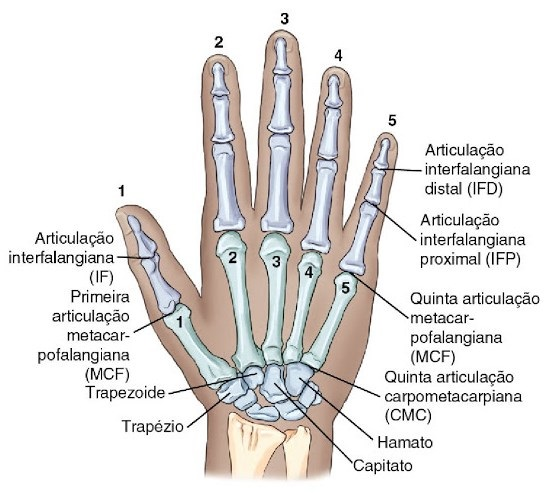
\includegraphics[width=.55\textwidth]{imagem/articulacoes}
  \captionsetup{justification=centering}
  \captionfont{\small{\textbf{\\Fonte: \citeonline{articulacoes}}}}
  \label{fig:art}
\end{figure}

\begin{figure}[H]
  \setlength{\abovecaptionskip}{0pt}
  \setlength{\belowcaptionskip}{0pt}
  \caption[Posições dos dedos para testes]{Posições dos dedos para testes}
  \centering
  \subfloat[1--4]{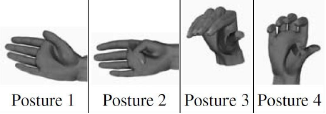
\includegraphics[width=.5\textwidth]{imagem/posicoes}\label{fig:pos1}}\\
  \subfloat[5--9]{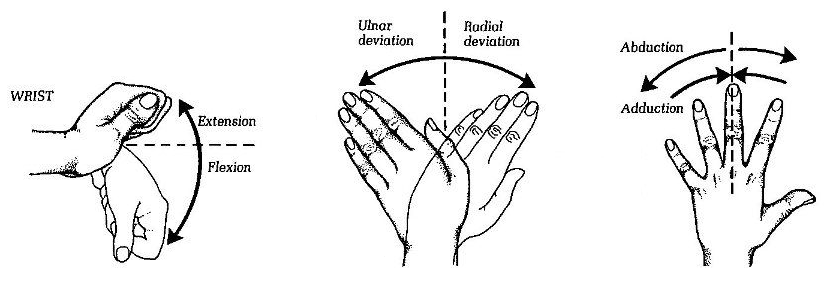
\includegraphics[width=.5\textwidth]{imagem/posicoes2}\label{fig:pos2}}
  \captionsetup{justification=centering}
  \captionfont{\small{\textbf{\\Fonte: \citeonline{li2009smartglove}, \citeonline{movimentos} (modificado pelo Autor)}}}
  \label{fig:pos}
\end{figure}

Para cada sensor e cada posição foi realizada uma análise estatística dos ângulos de dobra obtidos, calculando o \ac{DP} pela Equação \ref{eq:dp} e amplitude pela Equação \ref{eq:amp}, onde $X_S$ é o conjunto de amostras obtidas do sensor $S$ e $n$ é o número total de amostras. Por fim foi feita a média dos desvios padrão, amplitude e \ac{DMA} de cada sensor.

\begin{equation} \label{eq:dp}
	\delta_S = \sqrt{\frac{\sum_{i=1}^n(X_{S_i} - \overline{X_S})^2}{n-1}}
\end{equation}

\begin{equation} \label{eq:amp}
	R_S = \max(X_{S_i}) - \min(X_{S_i})
\end{equation}
